\documentclass[aspectratio=169,xcolor=dvipsnames]{beamer}
\usepackage{graphicx} % Required for inserting images
\pgfdeclareverticalshading[lower.bg,upper.bg]{bmb@transition}{200cm}{%
color(0pt)=(lower.bg); color(2pt)=(lower.bg); color(4pt)=(lower.bg)}

\setbeamersize{text margin left=2em,text margin right=2em}

\setbeamertemplate{footline}{
  \leavevmode%
  \hbox to \paperwidth{%
    \hfill%
    \usebeamerfont{footline}%
    \usebeamercolor[fg]{footline}%
    \insertframenumber/\inserttotalframenumber%
    \hspace{3em}%  % Adjust this value as needed
  }%
  \vskip2pt%
}
\setbeamertemplate{navigation symbols}{}

\setbeamertemplate{blocks}[rounded][shadow=false]

\setbeamertemplate{enumerate items}[default]
\setbeamertemplate{enumerate subitem}[default]
\setbeamertemplate{itemize items}[circle]
\setbeamertemplate{itemize subitem}[circle]

% table of contents (overview) settings
\setbeamertemplate{section in toc}[sections numbered]
\setbeamertemplate{subsection in toc}{%
    \leavevmode
    \leftskip=3.2em
    \rlap{\hskip-2em\inserttocsectionnumber.\inserttocsubsectionnumber}
    \inserttocsubsection\par
}

% frame title customization
\setbeamertemplate{frametitle}{%
    \vspace*{0.5em}
    \bfseries\insertframetitle\par
    \vskip-6pt
    \hrulefill\vspace{-0.1em}
}

% title page customization
\setbeamertemplate{title page}{%
    \vspace{2.5em}
    \begingroup
    \centering
    % ------------------------
    \begin{beamercolorbox}[sep=10pt,center]{title}
        \usebeamerfont{title}\inserttitle\par%
        \ifx\insertsubtitle\@empty%
        \else%
        \vskip 1em%
        {\usebeamerfont{subtitle}\usebeamercolor[fg]{subtitle}\insertsubtitle\par}%
        \fi%
    \end{beamercolorbox}%
    \vskip0.5em\par
    % ------------------------
    \begin{beamercolorbox}[sep=8pt,center]{author}
        \usebeamerfont{author}\insertauthor
    \end{beamercolorbox}
    \vskip1em
    % ------------------------
    \begin{beamercolorbox}[sep=8pt,center]{institute}
        \usebeamerfont{institute}\insertinstitute
    \end{beamercolorbox}\vskip0.5em
    % ------------------------
    \begin{beamercolorbox}[sep=8pt,center]{date}
        \usebeamerfont{date}\insertdate
    \end{beamercolorbox}\vskip1em
    % ------------------------
    {\usebeamercolor[fg]{titlegraphic}\inserttitlegraphic\par}
    \endgroup
    \vfill
}

\setbeamerfont{structure}{family=\sffamily,series=\mdseries}

\setbeamerfont{title}{size=\LARGE,series=\bfseries,parent=structure}
\setbeamerfont{subtitle}{size=\normalsize,parent=title}

\setbeamerfont{date}{size=\scriptsize,series=\mdseries,parent=structure}
\setbeamerfont{author}{size=\large,series=\mdseries,parent=structure}
\setbeamerfont{institute}{size=\scriptsize,series=\mdseries,parent=structure}

\setbeamerfont{section in toc}{size=\large,series=\bfseries,parent=structure}
\setbeamerfont{section in head/foot}{size=\tiny,parent=structure}
\setbeamerfont{subsection in toc}{size=\small,series=\mdseries,parent={section in toc}}

\setbeamerfont{frametitle}{size=\Large,series=\bfseries,parent=structure}
\setbeamerfont{framesubtitle}{parent=frametitle,size=\large}

\setbeamerfont{caption}{size=\footnotesize}
\setbeamerfont{item}{parent=structure,series=\mdseries}
\setbeamerfont{block title}{size=\large,series=\mdseries,parent={structure,block body}}

% Custom colors
\definecolor{MutedRed}{rgb}{0.97, 0.92, 0.92}
\definecolor{MutedGreen}{rgb}{0.92, 0.97, 0.92}
\definecolor{MutedBlue}{rgb}{0.92, 0.92, 0.97}
\definecolor{MutedBlack}{rgb}{0.95, 0.95, 0.95}

\definecolor{MediumRed}{rgb}{0.925, 0.345, 0.345}
\definecolor{MediumGreen}{rgb}{0.37, 0.7, 0.66}
\definecolor{MediumBlue}{rgb}{0.015, 0.315, 0.45}
\definecolor{MediumBlack}{rgb}{0.219, 0.259, 0.349}

\definecolor{DarkBlue}{rgb}{0.05, 0.15, 0.35}

% Set beamer color themes
\usecolortheme[named=DarkBlue]{structure}

% Customize block colors
\setbeamercolor{titlelike}{parent=structure}
\setbeamercolor{block title}{fg=white,bg=MediumBlue}
\setbeamercolor{block body}{fg=black,bg=MutedBlue}
\setbeamercolor{block title example}{fg=white,bg=MediumGreen}
\setbeamercolor{block body example}{fg=black,bg=MutedGreen}
\setbeamercolor{block title alerted}{fg=white,bg=MediumRed}
\setbeamercolor{block body alerted}{fg=black,bg=MutedRed}

% Environment for frames without page number
\newenvironment{hidepagenumberframe}
  {\setbeamertemplate{footline}{}\begin{frame}}
  {\end{frame}\setbeamertemplate{footline}[frame number]}

\usepackage{tikz}
\usetikzlibrary{arrows.meta, positioning, fit, backgrounds, calc, shapes.geometric, decorations.pathmorphing}

\setbeamertemplate{caption}[numbered]

\usepackage{booktabs}
\usepackage{array}
\usepackage{graphicx}
\usepackage{float}
\usepackage{amssymb}

\vspace{1.5em}

\begin{document}

\title{The Death of Distance: Internet and Political Trust in Africa}

\author[Illan Barriola, Rédha Chaba]{Illan Barriola\inst{1} \and Rédha Chaba\inst{2}}

\institute{
	\inst{1} CRED, Paris Panthéon Assas University, Paris, France
	\and
	\inst{2} LEMMA, Paris Panthéon Assas University, Paris, France
}
\date{June 26, 2025}

\begin{hidepagenumberframe}
    \titlepage
\end{hidepagenumberframe}

\addtocounter{framenumber}{-1}

\begin{frame}{Motivation}
\begin{itemize}
    \item Democracy requires citizens to both trust and distrust their politicians
    \vfill
    \begin{itemize}
        \item Trust to enable governance
        \vfill
        \item Distrust to prevent misgovernance
    \end{itemize}
    \vfill
\item In Sub-Saharan Africa: views of politicians and governments differ by region within countries
\vfill
    $\rightarrow$ People in remote areas tend to support them more than those near capital cities \textcolor{gray}{\textit{(Provenzano, 2024; Brinkerhoff et al., 2018)}}
\end{itemize}
\end{frame}


\begin{frame}{Greater support in remote regions}
\begin{itemize}
        \item State capacity diminishes in remote regions \textcolor{gray}{\textit{(Müller-Crepon, 2021; McKay et al., 2023)}}
        \vfill
    \begin{itemize}
        \item “\textit{The State stops twelve kilometers from the capital.}” (Bierschenk \& Olivier de \\
        \hspace{0.005em} Sardan, 1997)\\
        \vfill    
        $\rightarrow$ Citizens relate more to national institutions near capitals; remote areas maintain \\
        \hspace{1.1em} local/traditional focus \textcolor{gray}{\textit{(Herbst, 2000)}}\\
        \vfill
    \end{itemize}
\item Clientelist networks \textcolor{gray}{\textit{(Henn, 2023; Adida et al., 2020)}}
        \vfill
        \begin{itemize}
            \item More prevalent in remote regions where ethnic ties are stronger\\
            \vfill
        \end{itemize}
\item \textcolor[RGB]{220, 10, 10}{\textbf{Information gradient}} \textcolor{gray}{\textit{(Bhandari et al. 2023; Gottlieb, 2016)}}
\end{itemize}
\end{frame}

\begin{frame}{Information gradient}
\begin{itemize}
\item Information costs increase with distance from state presence and limited media coverage\\
\vfill
$\rightarrow$ Shortages of both direct and mediated information
\vfill
\item When information is scarce, citizens might end up trusting politicians in the absence of negative information
\end{itemize}
\end{frame}


\begin{frame}{Internet access}
\begin{itemize}
\item Mobile internet is changing traditional information geography in Sub-Saharan Africa
\vfill
\item Citizens in remote areas can now access diverse content that used to be concentrated near capitals
\vfill\begin{itemize}
    \vfill
    \item Including both political information
and misinformation
\end{itemize}
\vfill
\item Differs from traditional media by turning citizens from passive
consumers into active participants in different information networks
\vfill
\item \textcolor[RGB]{220, 10, 10}{\textbf{The impact on views of politicians is likely
to be larger in remote areas, where information costs have been highest}}
\end{itemize}
\end{frame}

\begin{frame}{Narrow spatial differences in political trust}
    \vspace{2em}
\centering    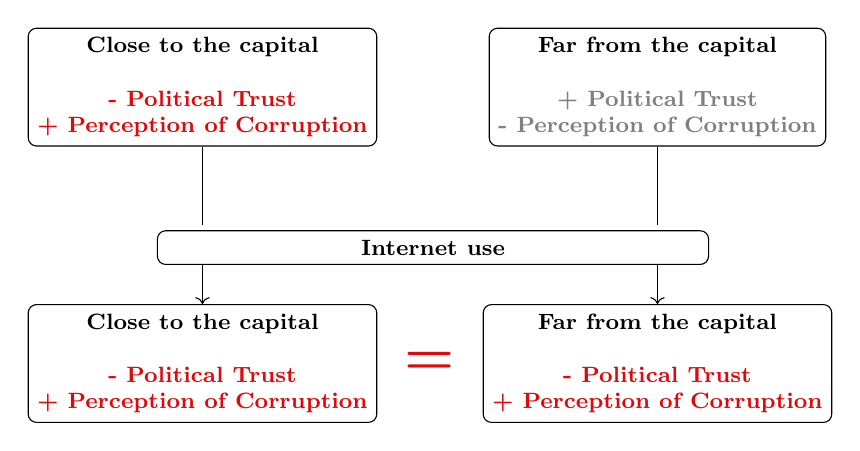
\begin{tikzpicture}
        \tikzset{
          node distance=5mm and 0mm,
          boite/.style={
            draw,align=center,
            font=\footnotesize\bfseries,text=black,
          },
          boite coins ronds/.style={boite,rounded corners=3pt},
          boite circulaire/.style={boite,circle},
          fleche/.style={
            line cap=round,-latex,line width=0.25mm,
          },
          grosse fleche/.style={fleche,line width=1mm},
          }
        \node[boite coins ronds, fill=white, below left=1cm] (a) {Close to the capital\\
        \vspace{0.01cm}\\
        \textcolor[RGB]{220, 10, 10}{- Political Trust}\\
        \textcolor[RGB]{220, 10, 10}{+ Perception of Corruption}};
        \node[boite coins ronds, fill=white, below right=1cm] (b) {Far from the capital\\
        \vspace{0.01cm}\\
        \textcolor{gray}{+ Political Trust}\\
        \textcolor{gray}{- Perception of Corruption}};
\node[boite coins ronds, fill=white, minimum width=7cm] (c) at (0,-3.5) {Internet use};
        \node[boite coins ronds,fill=white, below = 2cm of a] (d) {Close to the capital\\
        \vspace{0.01cm}\\
        \textcolor[RGB]{220, 10, 10}{- Political Trust}\\
        \textcolor[RGB]{220, 10, 10}{+ Perception of Corruption}};
        \node[boite coins ronds, fill=white, below=2cm of b] (e) {Far from the capital\\
        \vspace{0.01cm}\\
        \textcolor[RGB]{220, 10, 10}{- Political Trust}\\
        \textcolor[RGB]{220, 10, 10}{+ Perception of Corruption}};
            
        \begin{scope}[on background layer]
            \draw (a.south) -- ++(0,-1);
            \draw (b.south) -- ++(0,-1);
    \draw[->] (c.north -| a.south) -- (d.north -| a.south);
        \draw[->] (c.north -| b.south) -- (e.north -| b.south);
\node[font=\huge\bfseries] at ($(d.east)!0.5!(e.west)$) {\textcolor[RGB]{220, 10, 10}{=}};

        \end{scope}
      \end{tikzpicture}
\end{frame}

\begin{frame}{Related literature}
    \begin{itemize}
        \item Geography of trust\\
        \vfill
        \begin{itemize}
            \item McKay et al., 2019; Brinkerhoff et al. 2018; Yeandle, 2025\\
        \vfill
        \end{itemize}
        \item Internet and political behaviour\\
        \vfill
        \begin{itemize}
            \item Guriev et al. 2021; Cariolle et al. 2024; Manacorda and Tesei, 2020\\
        \vfill
        \end{itemize}
        \item Political economy of the capital city\\
        \vfill
        \begin{itemize}
            \item Provenzano, 2024; Michalopoulos and Papaioannou, 2014; Campante and Do, 2014\\
        \vfill
        \end{itemize}
    \end{itemize}
\end{frame}





\begin{frame}{Data}
\begin{columns}
\begin{column}{0.5\textwidth}
\begin{itemize}
    \item \textbf{Afrobarometer geocoded surveys}\\
    17 countries - Rounds 6-8 (2013-2021)
    \vspace{0.5em}
    \begin{itemize}
        \item Geolocated public opinion, media consumption, socio-demographics
        \vspace{0.5em}
        \item Distance calculations from capital cities
        \vspace{0.5em}
    \end{itemize}
    \vspace{0.5em}
    \item \textbf{GSMA internet coverage data}
    \vspace{0.5em}
    \begin{itemize}
        \item 3G coverage at 1×1-km resolution
     \vspace{0.5em}
        \item Aggregated to district level, weighted by population density
      \vspace{0.5em}
    \end{itemize}
    
\end{itemize}

\end{column}
\begin{column}{0.5\textwidth}
\begin{figure}
    \centering
    \includegraphics[width=0.9\textwidth]{C:/Users/Redha CHABA/Documents/wp_git/rbci/plots/discontinuity/cty_spl.jpg}
    \caption{Country Sample and Capital Cities}
\end{figure}
\end{column}
\end{columns}
\end{frame}



\begin{frame}{Internet and political trust}
\begin{equation}
    \fontsize{10}{11}\selectfont
    Trust_{irct} = \beta_{1} Dist_{irc} + \beta_{2} \textcolor[RGB]{220, 10, 10}{\textbf{Int\_use}_{rct}} + \beta_{3} \textcolor[RGB]{220, 10, 10}{\textbf{Dist} \times \textbf{Int\_use}_{irct}} + \Gamma X^{'}_{ir} + \mu_{ct}+ \varepsilon_{rt}
    \end{equation}
\vfill
\hspace{1em}
where\\
\vfill
    {\fontsize{10}{11}\selectfont
\begin{flushleft}
 \hspace{2.5em}
    - $Trust_{irct}$: average trust in president and parliament\\
    \vfill
\hspace{2.5em}
    - $Dist_{irc}$: normalized distance from the capital \textcolor{gray}{\textit{(Michalopoulos and Papaioannou, 2014)}}\\
    \vfill
 \hspace{2.5em}
   - \textcolor[RGB]{220, 10, 10}{\textbf{Int\_use}$_{rct}$:} district average of internet use\\
    \vfill
 \hspace{2.5em}
   - $X^{'}_{ir}$:
- Individual: socio-demographics, distances from largest non-capital city and roads, \\
\hspace{5.7em} traditional media consumption\\
\vfill
\hspace{5em}
- District: economic development, population density, area, terrain ruggedness, 2G \\
\hspace{5.7em} coverage president's birthplace\\    \vfill
\hspace{2.5em}
    - $\mu_{ct}$: country $\times$ time fixed effects\\ \vfill
\hspace{2.5em}
    - $\varepsilon_{rt}$: SE clustered at the region $\times$ time level



\end{flushleft}
    }
\end{frame}

\begin{frame}{Internet and political trust}
    \vfill
\begin{itemize}
    \item \textcolor[RGB]{220, 10, 10}{\textbf{Identification concerns:}} Reverse causality and unobserved factors
    \vfill
    \item \textcolor[rgb]{0.0,0.6,0.0}{\textbf{Instrumental variable:}} District average of 3G internet coverage weighted by population density \textcolor{gray}{(Guriev et al., 2021; Cariolle and Carroll, 2024)}\\
    \vfill
\end{itemize}

    \center
    
    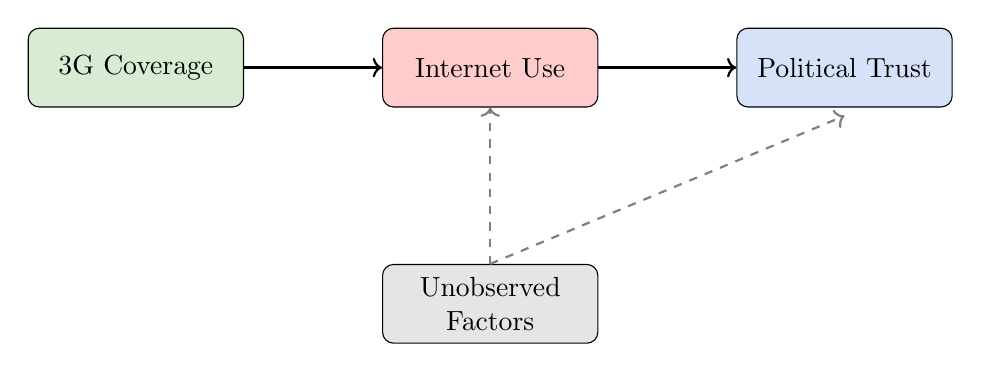
\begin{tikzpicture}[
    node distance=3cm,
    every node/.style={draw, rounded corners, text width=2.5cm, text centered, minimum height=1cm},
    arrow/.style={->, thick},
    red arrow/.style={->, thick, black},
    blue arrow/.style={->, thick, black},
    dashed arrow/.style={->, thick, dashed, gray}]

\node[fill={rgb,255:red,216;green,236;blue,212}] (instrument) at (0,2) {3G Coverage};
\node[fill=red!20] (treatment) at (4.5,2) {Internet Use};
\node[fill={rgb,255:red,214;green,226;blue,247}] (outcome) at (9,2) {Political Trust};
\node[fill=gray!20] (confounder) at (4.5,-1) {Unobserved Factors};

\draw[blue arrow] (instrument) -- (treatment);
\draw[red arrow] (treatment) -- (outcome);
\draw[dashed arrow] (confounder) -- (treatment);
\draw[dashed arrow] (confounder.north) -- ([yshift=-3pt]outcome.south);

\end{tikzpicture}


\end{frame}

    \begin{frame}{Internet and political trust}
        \begin{itemize}
\item 
3G supply location is determined by economic rather than political factors
\vfill
\begin{itemize}
    \item 
Particularly in Sub-Saharan Africa where costly internet infrastructure is mainly deployed by profit-focused private companies
\end{itemize}
\vfill
\item Population weighting and controls for economic development and topographic features help ensure the exogeneity of our instrument
\vfill
\item \textcolor{gray}{Robustness: We explore another framework using lightning strike patterns to instrument for 3G internet supply}
\end{itemize}
\end{frame}

    \begin{frame}{Internet and political trust}
    \centering \textbf{First-stage}
\vspace{0.5em}
    \begin{equation}
    \fontsize{10}{11}\selectfont
    \textcolor[RGB]{220, 10, 10}{\textbf{Int\_use}_{rct}} = \beta_{1} Dist_{irc} + \beta_{2} \textcolor[rgb]{0.0,0.6,0.0}{\textbf{3G\_coverage}_{rct}} + \Gamma X^{'}_{ir} + \mu_{ct}+ \varepsilon_{rt}
    \end{equation}
\\
\begin{equation}
    \fontsize{10}{11}\selectfont
    \textcolor[RGB]{220, 10, 10}{\textbf{Dist} \times \textbf{Int\_use}_{irct}} = \beta_{1} Dist_{irc} + \beta_{2} \textcolor[rgb]{0.0,0.6,0.0}{\textbf{Dist} \times \textbf{3G\_coverage}_{irct}} + \Gamma X^{'}_{ir} + \mu_{ct}+ \varepsilon_{rt}
    \end{equation}
\\
    \centering \textbf{Second-stage}
    \vspace{0.5em}
    \begin{equation}
    \fontsize{10}{11}\selectfont
    Trust_{irct} = \beta_{1} Dist_{irc} + \beta_{2}^{2S} \textcolor[rgb]{0.0,0.6,0.0}{\textbf{Int\_use}_{rct}} + \beta_{3}^{2S} \textcolor[rgb]{0.0,0.6,0.0}{\textbf{Dist} \times \textbf{Int\_use}_{irct}} + \Gamma X^{'}_{ir} + \mu_{ct}+ \varepsilon_{rt}
    \end{equation}

\end{frame}


\begin{frame}{Internet mitigates the distance effect}

\begin{figure}
    \includegraphics[scale=0.09]{C:/Users/Redha CHABA/Documents/wp_git/rbci/plots/marginal_effect/int_use_adm/pol_trust_iv_10p.jpg}
    \caption{Marginal effect of distance from the capital as a function of internet use}
\end{figure}

\end{frame}

\begin{frame}{Internet mitigates the distance effect}
    \begin{table}[H]
    \centering
    \resizebox{10.5cm}{!}{
    \begin{tabular}{@{\extracolsep{5pt}} l c c c c c c}
    \\
    \toprule
    \toprule
    & \multicolumn{1}{c}{{OLS}} & \multicolumn{3}{c}{{First Stage}} & \multicolumn{1}{c}{{2SLS}}\\
        \cmidrule(r){2-2}
        \cmidrule(r){3-5}
        \cmidrule(r){6-6}
        & \multicolumn{1}{c}{{Pol. trust}} & \multicolumn{1}{c}{{Dist. $\times$ Int. use}} & \multicolumn{1}{c}{{}} &  \multicolumn{1}{c}{{Int. use}} & \multicolumn{1}{c}{{Pol. trust}}\\
        \cmidrule(r){2-2}
        \cmidrule(r){3-3}
        \cmidrule(r){5-5}    
        \cmidrule(r){6-6}    
        & \multicolumn{1}{c}{{(1)}} & \multicolumn{1}{c}{{(2)}} & \multicolumn{1}{c}{{}} &  \multicolumn{1}{c}{{(3)}} & \multicolumn{1}{c}{{(4)}}\\
        
        \midrule
  

Distance from the capital&      0.514***&&&&       0.513***\\
\smallskip
&       (0.06)  &&&&      (0.09)   \\
Distance from the capital $\times$ Internet use&    -0.423***&&&&      -0.628***         \\
\smallskip
&       (0.09)   &&&&      (0.16)  \\
Internet use&     0.081*&&&&      -0.306        \\
\smallskip
        &     (0.05)   &&&&        (0.19)           \\



Distance from the capital city $\times$ 3G coverage&&0.733***  && -0.048\\
        \smallskip&& (0.06) &&  (0.10) \\
3G coverage &&-0.086***&&0.330***  \\
\medskip&& (0.02) && (0.05)\\

     \midrule
     SW \emph{F} - Distance $\times$ 3G coverage &-&-& 258.6 &-&-\\
     \smallskip
    SW \emph{F} - 3G coverage &-&-& 50.65 &-&-\\
    \smallskip
    Country X Round FE       & \checkmark & \checkmark&- & \checkmark & \checkmark \\
    Individual \& district controls  & \checkmark & \checkmark & - &  \checkmark & \checkmark\\
    \smallskip
    Observations       &       66,574    &66,574 & &       66,574 & 66,574  \\
    Adjusted-R$^2$    &       0.178     &-&-&-&-  \\
                          \bottomrule
    \multicolumn{6}{p{18cm}}{}
\end{tabular}}
    \caption{Effect of internet use on political trust by distance}

    \end{table}

\end{frame}


\begin{frame}{Internet mitigates the distance effect}
    \begin{itemize}
        \item Internet use shifts opinions in remote areas towards the critical views found near
capitals
\vfill
        \item We cannot disentangle whether citizens consume accurate information or misinformation\\
        \vfill
        $\rightarrow$ We explore institutional heterogeneity: traditional media freedom and corruption indexes
    \end{itemize}
\end{frame}

\begin{frame}{More pronounced where the state controls traditional media}
        \begin{figure}
    \centering
    \includegraphics[width=0.65\textwidth]{C:/Users/Redha CHABA/Documents/wp_git/rbci/plots/marginal_effect/int_use_adm/rsf_iv_10p.jpg}
    \caption{Political Trust - Media Freedom}
\end{figure}
\end{frame}


\begin{frame}{Where there is corruption}
        \begin{figure}
    \centering
    \includegraphics[width=0.65\textwidth]{C:/Users/Redha CHABA/Documents/wp_git/rbci/plots/marginal_effect/int_use_adm/pol_corr_gici_iv_10p.jpg}
    \caption{Political Corruption - Corruption Index}
\end{figure}
\end{frame}


\begin{frame}{Country heterogeneity}
    
\begin{table}[H]
    \centering
    \resizebox{10cm}{!}{
    \begin{tabular}{@{\extracolsep{5pt}} l c c c c}
    \\
    \toprule
    \toprule
        & \multicolumn{2}{c}{{Pol. Trust}} & \multicolumn{2}{c}{{Pol. Corr}}\\
        \cmidrule(r){2-3}
        \cmidrule(r){4-5}
        & \multicolumn{2}{c}{{Media}} & \multicolumn{2}{c}{{Corruption}}\\
        \cmidrule(r){2-3}
        \cmidrule(r){4-5}
        & \multicolumn{1}{c}{{Free}} & \multicolumn{1}{c}{{Captured}} & \multicolumn{1}{c}{{Low}} & \multicolumn{1}{c}{{High}}\\
        \cmidrule(r){2-2}
        \cmidrule(r){3-3}
        \cmidrule(r){4-4}
        \cmidrule(r){5-5}
        & \multicolumn{1}{c}{{(1)}} & \multicolumn{1}{c}{{(2)}} & \multicolumn{1}{c}{{(3)}} &  \multicolumn{1}{c}{{(4)}}\\
        
        \midrule
  


Distance from the capital        &      0.455***&       0.722***&           -0.533***&      -0.775***\\
\smallskip
&     (0.13)   &      (0.18)   &      (0.11)   &      (0.09)  \\
Distance from the capital $\times$ Int. use&      -0.250   &      -0.826***&         0.700** &       1.032***\\
\smallskip            &       (0.25)   &      (0.24)  &      (0.32)   &      (0.27)   \\

Internet use &       -0.262   &       0.047   &           -0.286   &      -0.687** \\
\medskip            &      (0.29)   &      (0.35)     &        (0.41)   &      (0.30)   \\


     \midrule
    Country X Round FE       & \checkmark & \checkmark & \checkmark & \checkmark \\
    Individual \& district controls   & \checkmark & \checkmark & \checkmark & \checkmark \\
    Geographic controls  & \checkmark & \checkmark & \checkmark & \checkmark  \\
    \smallskip
    Observations        &       31,210   &       35,364   &       17,745   &       44,633  \\
                          \bottomrule
    \multicolumn{5}{p{14cm}}{}
\end{tabular}}
    \caption{Media freedom and corruption level}
    \end{table}

\end{frame}


\begin{frame}{When education is low}
        \begin{figure}
    \centering
    \includegraphics[width=0.65\textwidth]{C:/Users/Redha CHABA/Documents/wp_git/rbci/plots/marginal_effect/int_use_adm/educ_iv_10p.jpg}
    \caption{Political Trust - Education Level}
\end{figure}
\end{frame}

\begin{frame}{Individual heterogeneity}

        \begin{table}[H]
    \centering
    \resizebox{12cm}{!}{
    \begin{tabular}{@{\extracolsep{5pt}} l c c c c c}
    \\
    \toprule
    \toprule
    & \multicolumn{2}{c}{{Education}} & \multicolumn{3}{c}{{Age}}\\
        \cmidrule(r){2-3}
        \cmidrule(r){4-6}
        & \multicolumn{1}{c}{{High}} & \multicolumn{1}{c}{{Low}} & \multicolumn{1}{c}{{18-25}} & \multicolumn{1}{c}{{26-40}} & \multicolumn{1}{c}{{41+}}\\
        \cmidrule(r){2-2}
        \cmidrule(r){3-3}
        \cmidrule(r){4-4}
        \cmidrule(r){5-5}
        \cmidrule(r){6-6}

        & \multicolumn{1}{c}{{(1)}} & \multicolumn{1}{c}{{(2)}} & \multicolumn{1}{c}{{(3)}} &  \multicolumn{1}{c}{{(4)}} &  \multicolumn{1}{c}{{(5)}}\\
        
        \midrule


Distance from the capital        &      0.402** &       0.594***&       0.801***&       0.495***&       0.387***\\
\smallskip
            &     (0.16)   &      (0.11)               &     (0.13)   &      (0.12)   &      (0.12)   \\


Distance from the capital $\times$ Int. use&      -0.348*  &      -0.788***&      -0.916***&      -0.526***&      -0.501** \\
\smallskip            &     (0.21)   &      (0.21)              &     (0.19)   &      (0.18)   &      (0.21)   \\
Internet use &       -0.341   &      -0.167  &        0.019   &      -0.379   &      -0.473** \\
\medskip            &       (0.23)   &      (0.20)  &       (0.22)   &      (0.23)   &      (0.24)   \\

     \midrule
    Country X Round FE       & \checkmark & \checkmark & \checkmark & \checkmark & \checkmark \\
    Individual \& district controls   & \checkmark & \checkmark & \checkmark & \checkmark  & \checkmark\\
    Geographic controls  & \checkmark & \checkmark & \checkmark & \checkmark  & \checkmark\\
    \smallskip
    Observations        &         20,428   &       46,146  &       17,519   &       27,607   &       21,614   \\
                          \bottomrule
    \multicolumn{5}{p{13cm}}{}
\end{tabular}}
    \caption{Political Trust - Individual Heterogeneity}

    \end{table}

\end{frame}

\begin{frame}{Other political outcomes}

        \begin{table}[H]
    \centering
    \resizebox{12cm}{!}{
    \begin{tabular}{@{\extracolsep{5pt}} l c c c c}
    \\
    \toprule
    \toprule
    & \multicolumn{1}{c}{{Perf. Econ.}} & \multicolumn{1}{c}{{Account. Citizens}} & \multicolumn{1}{c}{{Account. Parl.}} & \multicolumn{1}{c}{{Vote Oppo.}}\\
        \cmidrule(r){2-2}
        \cmidrule(r){3-3}
        \cmidrule(r){4-4}
        \cmidrule(r){5-5}
        & \multicolumn{1}{c}{{(1)}} & \multicolumn{1}{c}{{(2)}} & \multicolumn{1}{c}{{(3)}} &  \multicolumn{1}{c}{{(4)}}\\
        
        \midrule

Distance from the capital         &       0.339***&      -0.099** &      -0.098** &       0.184** \\
\smallskip
            &      (0.10)   &      (0.04)   &      (0.04)   &      (0.07)   \\

Distance from the capital $\times$ Int. use&      -0.222** &       0.110** &       0.108** &      -0.178** \\
\smallskip
 &      (0.10)   &      (0.05)   &      (0.04)   &      (0.08)   \\
Internet use&       0.148   &      -0.037   &      -0.037   &      -0.063   \\
\medskip                        &      (0.11)   &      (0.05)   &      (0.05)   &      (0.08)   \\


     \midrule
    Country X Round FE       & \checkmark & \checkmark & \checkmark & \checkmark\\
    Individual \& district controls   & \checkmark & \checkmark & \checkmark & \checkmark\\
    Geographic controls  & \checkmark & \checkmark & \checkmark & \checkmark\\
    \smallskip
    Observations        &       65,364   &       66,612   &       65,728   &       45,329   \\
                          \bottomrule
    \multicolumn{5}{p{13cm}}{}
\end{tabular}}
    \caption{Other political outcomes}

    \end{table}

\end{frame}



\begin{frame}{Robustness}
\begin{itemize}
    \item Distance measures: km, log(km), mean normalization, excluding closest/furthest observations
    \vfill
    \item Geographical IV: Lightning strikes
    \vfill
    \item Leave-one-out regressions: Estimated coefficient and AR Weak IV test
\end{itemize}
    

\end{frame}

\begin{frame}{Conclusion}
    \begin{enumerate}
        \item \textcolor[RGB]{220, 10, 10}{\textbf{Internet use shifts opinions in remote areas}} towards the critical views found near capitals
        \vfill
        \item The reduction in spatial disparities in political trust is more pronounced in countries with \textcolor[RGB]{220, 10, 10}{\textbf{high corruption and where the state controls traditional media}}\\
        \vfill
        $\rightarrow$ Supports "liberation technology" arguments that the internet offers alternative information when traditional media are not transparent
        \vfill
        \item These attitude changes translate into \textcolor[RGB]{220, 10, 10}{\textbf{increased government accountability demands}} and opposition voting
    \end{enumerate}
\end{frame}

\begin{frame}{Next steps}
    \begin{itemize}
        \item Language: traditional media could be in a language that's difficult to access, while the internet can provide content in local languages
        \vfill
        \item Differences in internet news/use/social media news
        \vfill
        \item Positive/Negative events heterogeneity
        \vfill
        \item Submarine cables instrument
        \vfill
        \item Staggered DiD specification
        \vfill
        \item 0.5 $\times$ 0.5° grid focus
        \vfill
    \end{itemize}
\end{frame}

\begin{frame}
    \begin{center}
        \Large Thank you!\\
        \vspace{1em}
        \textcolor{DarkBlue}{Illan.Barriola@assas-universite.fr}\\
        \vspace{1em}
        \textcolor{DarkBlue}{Redha.Chaba@assas-universite.fr}
    \end{center}
\end{frame}





\begin{frame}[noframenumbering]{Distance and political trust}
\begin{equation}
    \fontsize{10}{11}\selectfont
    Trust_{irct} = \beta_{1} Dist_{irc} + \Gamma X^{'}_{ir} + \mu_{ct}+ \varepsilon_{rt}
    \end{equation}
\vfill
\hspace{1em}
where\\
\vfill
    {\fontsize{9}{12}\selectfont
\begin{flushleft}
\hspace{2.5em}
    - $Trust_{irct}$: average trust in president and parliament\\
    \vfill
\hspace{2.5em}
    - $Dist_{irc}$: normalized distance from the capital \textcolor{gray}{\textit{(Michalopoulos and Papaioannou, 2014)}}\\
    \vfill
 \hspace{2.5em}
   - $X^{'}_{ir}$: individual and district controls\\ \vfill
 \hspace{5em}
- Individual: socio-demographics, distances from largest non-capital city and roads, traditional\\
 \hspace{10.3em}
 media consumption\\
\hspace{5em}
- District: economic development, population density, area, president's birthplace\\    \vfill
\hspace{2.5em}
    - $\mu_{ct}$: country $\times$ time fixed effects\\ \vfill
\hspace{2.5em}
    - $\varepsilon_{rt}$: SE clustered at the region $\times$ time level
\end{flushleft}
    }
\end{frame}



\begin{frame}[noframenumbering]{Distance and political trust}
    \begin{columns}
    \begin{column}{0.5\textwidth}
        \begin{figure}
    \centering
    \includegraphics[width=0.825\textwidth]{C:/Users/Redha CHABA/Documents/wp_git/rbci/plots/discontinuity/murdock_map.jpg}
    \caption{Ethnic Areas and National Boundaries}
\end{figure}
    \end{column}

    \begin{column}{0.5\textwidth}
        \begin{figure}
    \centering
    \includegraphics[width=0.385\textwidth]{C:/Users/Redha CHABA/Documents/wp_git/rbci/plots/discontinuity/benin_niger.jpg}
    \caption{Example: Dendi Ethnic Group}
\end{figure}

    \end{column}

\end{columns}
\end{frame}




\begin{frame}[noframenumbering]{Distance and political trust}
    \centering \textcolor[rgb]{0.0,0.6,0.0}{\textbf{Identification assumptions}}\vfill
    \setbeamertemplate{enumerate items}[default]
    \begin{enumerate}
        \item Two individuals living in the same historical ethnic group share similar characteristics, with distance from capital as the key differentiating factor \\ \vfill
        \textcolor{gray}{\textit{Michalopoulos and Papaioannou, 2014; Provenzano, 2024; McCauley and Posner, 2015}} \\ \vfill
        \begin{equation}
    Trust_{irct}=\beta_{1}Dist_{irc}+\Gamma X^{'}_{ir}+ \mu_{ct} + \textcolor[rgb]{0.0,0.6,0.0}{\mathbf{\nu_{e}}}+\varepsilon_{ict}
    \end{equation}\vfill
        \item Cross-border variation in trust reflects distance effects rather than institutional differences between countries
        
\begin{equation}
    Trust_{irct}=\beta_{1}Dist_{irc}+\Gamma X^{'}_{ir}+ \textcolor[rgb]{0.0,0.6,0.0}{\theta Z^{'}_{ct}} + \textcolor[rgb]{0.0,0.6,0.0}{\mathbf{\nu_{e}}}+\textcolor[rgb]{0.0,0.6,0.0}{\lambda_{t}}+\varepsilon_{ict}
    \end{equation}
            
    \end{enumerate}
\end{frame}


\begin{frame}[noframenumbering]{Distance increases political trust}

\begin{figure}
    \includegraphics[scale=0.15]{C:/Users/Redha CHABA/Documents/wp_git/rbci/plots/discontinuity/df_25_fe.jpg}
    \caption{Border discontinuity - \textit{Based on regression estimates from (2) of Table 1}}
\end{figure}

\end{frame}


\begin{frame}[noframenumbering]{Distance increases political trust}
    
    \begin{table}[H]
    \centering
    \resizebox{10cm}{!}{
    \begin{tabular}{@{\extracolsep{5pt}} l c c c}
    \\
    \toprule
    \toprule
    & \multicolumn{1}{c}{{Base sample}} & \multicolumn{2}{c}{{Border sample (25km)}} \\
        \cmidrule(r){2-2}
        \cmidrule(r){3-4}
        & \multicolumn{1}{c}{{(1)}} & \multicolumn{1}{c}{{(2)}} & \multicolumn{1}{c}{{(3)}}\\
        \midrule
  

Distance from the capital   &       0.311***&       0.547** &       0.845***\\
\medskip
            &      (0.04)   &      (0.22)   &      (0.21)   \\


     \midrule
    Country X Round FE       & \checkmark & \checkmark & $\times$\\
    Country controls       & $\times$ & $\times$ & \checkmark\\
    Individual \& district controls   & \checkmark & \checkmark & \checkmark \\
    \smallskip
    Observations        &       66,574   &        5,494   &        5,494   \\
    Adjusted-R$^2$           &         0.176   &       0.168   &       0.139   \\
                          \bottomrule
    \multicolumn{4}{p{11cm}}{}
\end{tabular}}
    \caption{Effect of distance from the capital on political trust}
\end{table}

\end{frame}



\begin{frame}[noframenumbering]{Political corruption}
        \begin{figure}
    \centering
    \includegraphics[width=0.65\textwidth]{C:/Users/Redha CHABA/Documents/wp_git/rbci/plots/marginal_effect/int_use_adm/pol_corr_iv_10p.jpg}
    \caption{Political corruption perception}
\end{figure}
\end{frame}

\begin{frame}[noframenumbering]{Political corruption perception}
    
        \begin{table}[H]
    \centering
    \resizebox{7cm}{!}{
    \begin{tabular}{@{\extracolsep{5pt}} l c}
    \\
    \toprule
    \toprule
    & \multicolumn{1}{c}{{Pol. Corr}}\\
        \cmidrule(r){2-2}
        & \multicolumn{1}{c}{{(1)}}\\
        
        \midrule

Distance from the capital        &            -0.377***\\
\smallskip
            &      (0.07)   \\

Distance from the capital $\times$ Int. use &        0.522***\\
\smallskip
            &      (0.12)   \\

Internet use &       -0.154    \\
\medskip
            &      (0.16)   \\



     \midrule
    Country X Round FE       & \checkmark\\
    Individual \& district controls   & \checkmark\\
    Geographic controls  & \checkmark\\
    \smallskip
    Observations        &       62,378 \\
                          \bottomrule
    \multicolumn{2}{p{8cm}}{}
\end{tabular}}
    \caption{Political corruption perception}

    \end{table}

\end{frame}

\begin{frame}[noframenumbering]{Economic performance}
        \begin{figure}
    \centering
    \includegraphics[width=0.65\textwidth]{C:/Users/Redha CHABA/Documents/wp_git/rbci/plots/marginal_effect/int_use_adm/perf_eco_iv_10p.jpg}
    \caption{Economic performance}
\end{figure}
\end{frame}


\begin{frame}[noframenumbering]{Accoutability towards citizens}
        \begin{figure}
    \centering
    \includegraphics[width=0.65\textwidth]{C:/Users/Redha CHABA/Documents/wp_git/rbci/plots/marginal_effect/int_use_adm/check_citiz_iv_10p.jpg}
    \caption{Accoutability towards citizens}
\end{figure}
\end{frame}

\begin{frame}[noframenumbering]{Accoutability towards parliament}
        \begin{figure}
    \centering
    \includegraphics[width=0.65\textwidth]{C:/Users/Redha CHABA/Documents/wp_git/rbci/plots/marginal_effect/int_use_adm/check_parl_iv_10p.jpg}
    \caption{Accoutability towards parliament}
\end{figure}
\end{frame}

\begin{frame}[noframenumbering]{Willingness to vote for the ruling party}
        \begin{figure}
    \centering
    \includegraphics[width=0.65\textwidth]{C:/Users/Redha CHABA/Documents/wp_git/rbci/plots/marginal_effect/int_use_adm/vote_oppo_min_iv_10p.jpg}
    \caption{Willingness to vote for the ruling party}
\end{figure}
\end{frame}

\end{document}
